\documentclass[dvipdfmx]{jarticle}
\usepackage{graphicx}
\usepackage[top=30truemm,bottom=30truemm,left=25truemm,right=25truemm]{geometry}
\usepackage{listings,jvlisting}
\usepackage{url}
\title{計算機援用工学前半レポート}
\author{ソフトウェア科学コース\\09B22084山久保孝亮}
\date{\today}


\lstset{
  basicstyle={\ttfamily},
  identifierstyle={\small},
  commentstyle={\smallitshape},
  keywordstyle={\small\bfseries},
  ndkeywordstyle={\small},
  stringstyle={\small\ttfamily},
  frame={tb},
  breaklines=true,
  columns=[l]{fullflexible},
  numbers=left,
  xrightmargin=0zw,
  xleftmargin=3zw,
  numberstyle={\scriptsize},
  stepnumber=1,
  numbersep=1zw,
  lineskip=-0.5ex
}

\begin{document}
\maketitle
今回私が選んだ授業で出てくるワードは暗号化技術である.特に,POODLEによるSSLv3の脆弱性について詳しく調査した.
\section{選んだ理由}
私がこのテーマを選んだ理由としては,この脆弱性が原因でガラケーからスマホへの移行が進んだという授業内の話に関心を持ったためである.
\section{調査の概要}
\subsection{技術の背景}
SSLv3は暗号化通信用のプロトコルであり,ドコモ,au,ソフトバンクなどのキャリアが提供するiモードブラウザ等でサポートされていた.\cite{0}
SSLv3で利用される暗号はCBC方式のブロック暗号を選択することができ,以下の図1のように一定のサイズのブロックごとに暗号化・復号を行う.
\begin{figure}[h]
    \centering
    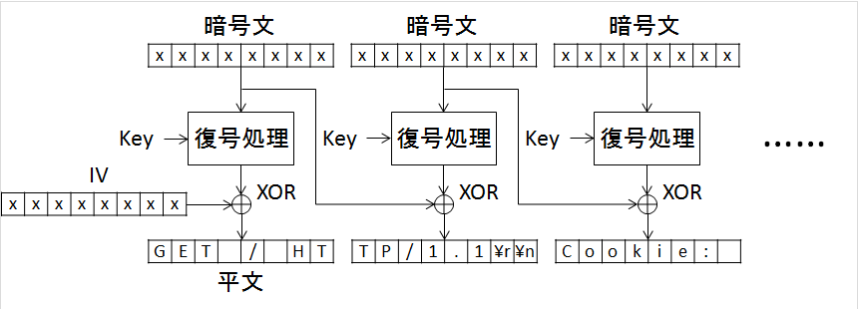
\includegraphics[width = 8cm]{CBC.png}
    \caption{ブロック暗号の復号処理}
\end{figure}
\\一定サイズごとに復号を行うため,平文の最後がブロック長に比べて中途半端な長さになることが発生してしまう.その場合はダミーの文字を入れて調整を行っていた.
この調整のために平文の最後に追加される文字をPaddingという.また,一番最後のバイトはPadding長として規定されており,例えば平文がブロックサイズちょうどであっても,Padding長を格納するために
ダミー文字とPadding長のみのブロックが追加されていた.そしてこのPadding長を使って復号の際に何文字Paddingを無視するかを判断していた.
\subsection{手法}
POODLEでは2.1で例として挙げたPaddingのみで構成されるブロックを使用してほかのブロックの平文の推測を行う.具体的には,
\subsection{結果}

\section{自分の見解}

\begin{thebibliography}{99}
    \bibitem{0} \url{https://qiita.com/harukasan/items/dee779c0a3f624758230} 12/16アクセス
    \bibitem{1} \url{https://engineering.dena.com/blog/2014/10/poodle/} 12/16アクセス
\end{thebibliography}
\end{document}